\section{Patterns}

\subsection{Dependencies}

\definition{Dependencies} are critical when designing parallel programs as they directly influence the program's correctness and potential for parallelism.

\begin{definitionbox}
    A \textbf{dependency} arises when one operation depends on an earlier operation to complete and produce a result before this later operation can be performed.
\end{definitionbox}

\noindent
Non-directly, dependencies \textbf{determine the order in which operations must be executed to maintain correctness}.

\highspace
\begin{flushleft}
    \textcolor{Green3}{\faIcon{question-circle} \textbf{Why is sequential consistency important?}}
\end{flushleft}
\definition{Sequential Consistency} ensures that the results of a parallel program's execution are as if the operations of all processors were executed in some sequential order, while preserving the program order for each processor. It is so important because:
\begin{itemize}
    \item \important{Enforcing Dependencies}:
    \begin{itemize}
        \item \textbf{Ordered Execution}. Sequential consistency ensures that operations are executed in an order that respects their dependencies.

        \item \textbf{Data Integrity}. By maintaining the correct order of dependent operations, \hl{sequential consistency preserves the integrity of the data being manipulated in parallel programs}.
    \end{itemize}

    \item \important{Predictable Behavior}:
    \begin{itemize}
        \item \textbf{Program Order Preservation}. Dependencies define the required order of operations within a program. Sequential consistency ensures each processor's operations appear in sequence, respecting these dependencies.

        \item \textbf{Non-Interference}. Sequential consistency \hl{guarantees that operations from different processors can interleave their executions in many possible sequences}, but the \hl{final results are consistent with some sequential execution that respects dependencies}.
    \end{itemize}
\end{itemize}
This type of model has already been discussed in Section \ref{subsection: Sequential Consistency Model} on page \pageref{subsection: Sequential Consistency Model}. However, we can summarize the guarantees it provides:
\begin{itemize}[label=\textcolor{Green3}{\faIcon{check}}]
    \item \textcolor{Green3}{\textbf{Simplified Reasoning}}. Programmers can reason about parallel programs more easily, as if they were sequential.
    \item \textcolor{Green3}{\textbf{Correctness}}. It helps maintain the correctness of shared memory operations in concurrent programs.
\end{itemize}

\newpage

\begin{flushleft}
    \textcolor{Green3}{\faIcon{question-circle} \textbf{How to detect dependencies?}}
\end{flushleft}
By identifying where dependencies occur, we can determine where operations need to be synchronized or reordered to ensure accurate results. But the real dilemma is, \dquotes{\emph{how do we know when two or more statements are interdependent?}}. The short answer is: it is not always that easy. It depends on the complexity of the code, but in general, the definitions are as follows:
\begin{itemize}
    \item \definition{Independent Statements}: two statements are independent if their \textbf{execution order does not affect the computation outcome}.

    The implication is that the order of execution is interchangeable without changing the final state.


    \item \definition{Dependent Statements}: statements are dependent if the \textbf{order of their execution impacts the computation result}.

    The implication is that changing the order of execution alters the final outcome, so the sequence of operations matters.
\end{itemize}

\highspace
\begin{flushleft}
    \textcolor{Green3}{\faIcon{stream} \textbf{Type of dependencies}}
\end{flushleft}
Dependencies can be categorized into several types:
\begin{itemize}
    \item \definition{Control Dependencies}: execution of one operation depends on the control flow (like \texttt{if} statements or loops).

    \item \definition{Data Dependencies}: one operation requires the result of another operation:
    \begin{itemize}
        \item \definition{True Dependency} (Read After Write, RAW): a subsequent operation reads data after it's written.
        \item \definition{Anti-Dependency} (Write After Read, WAR): a write operation must occur after all preceding read operations.
        \item \definition{Output Dependency} (Write After Write, WAW): two write operations must occur in a particular sequence.
    \end{itemize}
\end{itemize}

\highspace
\begin{examplebox}[: Dependencies]
    Some dependency scenarios:
    \begin{itemize}
        \item \textbf{Independent Statements}
        \begin{itemize}
            \item Statement 1: \texttt{a=1;}
            \item Statement 2: \texttt{b=1;}
        \end{itemize}
        Since these two statements do not rely on each other's values, they are independent. Executing them in any order does not change the outcome.

        \newpage

        \item \textbf{True (flow) Dependency}
        \begin{itemize}
            \item Statement 1: \texttt{a=1;}
            \item Statement 2: \texttt{b=a;}
        \end{itemize}
        \texttt{S2} depends on the value of \texttt{a} from \texttt{S1}. This is a true (or flow) dependency, as \texttt{S2} requires \texttt{S1} to execute first to produce the correct result.

        \item \textbf{Output Dependency}
        \begin{itemize}
            \item Statement 1: \texttt{a=f(x);}
            \item Statement 2: \texttt{a=b;}
        \end{itemize}
        Both statements write to \texttt{a}, creating an output dependency. The order matters because both statements affect the value of \texttt{a}.
        
        \item \textbf{Anti-Dependency}
        \begin{itemize}
            \item Statement 1: \texttt{a=b;}
            \item Statement 2: \texttt{b=1;}
        \end{itemize}
        There is an anti-dependency where \texttt{S1} reads \texttt{b}, and \texttt{S2} writes to \texttt{b}. The execution order affects the value read by \texttt{S1}.
    \end{itemize}
\end{examplebox}

\highspace
\begin{flushleft}
    \textcolor{Green3}{\faIcon{tools} \textbf{Dependency Graph}}
\end{flushleft}
Dependencies can be represented as a graph, also known as a \definition{dependency graph}.
\begin{itemize}
    \item \textbf{Nodes (statements)}. Each node represents a statement in the program. For example:
    \begin{itemize}
        \item Statement 1: \texttt{a = 1;}
        \item Statement 2: \texttt{b = a;}
        \item Statement 3: \texttt{a = b + 1;}
        \item Statement 4: \texttt{c = a;}
    \end{itemize}
    The dependency graph is:
    \begin{center}
        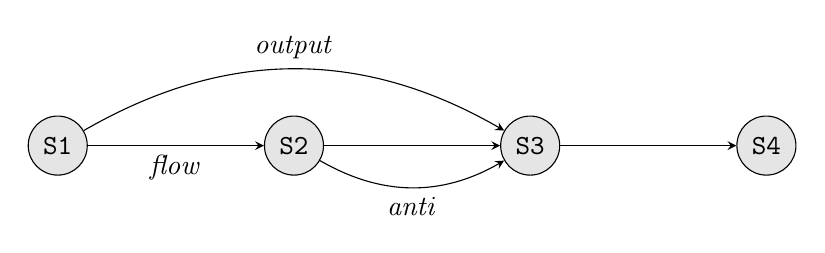
\begin{tikzpicture}[->, >=stealth, node distance=3cm]
            \tikzstyle{state} = [circle, draw, fill=gray!20, text centered, minimum height=2em]

            % Nodes
            \node[state] (S1) {\texttt{S1}};
            \node[state] (S2) [right of=S1] {\texttt{S2}};
            \node[state] (S3) [right of=S2] {\texttt{S3}};
            \node[state] (S4) [right of=S3] {\texttt{S4}};

            % Edges
            \path (S1) edge [bend left] node[above] {\emph{output}} (S3);
            \path (S1) edge node[below] {\emph{flow}} (S2);
            \path (S2) edge (S3);
            \path (S2) edge [bend right] node[below] {\emph{anti}} (S3);
            \path (S3) edge (S4);

        \end{tikzpicture}
    \end{center}

    \item \textbf{Edges (dependencies)}. Arrows between nodes indicate dependencies between statements. Here are the key types of dependencies shown (in the previous dependency graph):
    \begin{itemize}
        \item \important{True (flow) dependency}:
        \begin{equation*}
            \texttt{S2} \hspace{1em} \delta \hspace{1em} \texttt{S3}
        \end{equation*}
        An arrow from \texttt{S2} to \texttt{S3} signifies that \texttt{S3} depends on \texttt{S2} for the value of \texttt{a}.
        \item \important{Output dependency}:
        \begin{equation*}
            \texttt{S1} \hspace{1em} \delta^{0} \hspace{1em} \texttt{S3}
        \end{equation*}
        An arrow from \texttt{S1} to \texttt{S3} indicates that both \texttt{S1} and \texttt{S3} write to \texttt{a}.
        \item \important{Anti dependency}:
        \begin{equation*}
            \texttt{S2} \hspace{1em} \delta^{-1} \hspace{1em} \texttt{S3}
        \end{equation*}
        An arrow from \texttt{S2} to \texttt{S3} shows that \texttt{S2} reads \texttt{a}, while \texttt{S3} writes to \texttt{a}.
    \end{itemize}
\end{itemize}

\highspace
\begin{flushleft}
    \textcolor{Green3}{\faIcon{question-circle} \textbf{Why do we compute dependencies?}}
\end{flushleft}
Computing data dependencies is important for several reasons, such as optimizing code (compilers can reorder or optimize code better if they know which statements depend on each other), avoiding data hazards (in hardware design, understanding dependencies is essential to avoid hazards), debugging and maintenance (understanding dependencies helps debugging by showing how data flows through the program), etc.

\highspace
Therefore, by \textbf{computing data dependencies, we get a clear picture of how data is used and modified throughout the program}. This systematic approach can lead to more efficient, reliable, and maintainable code.

\highspace
\begin{flushleft}
    \textcolor{Green3}{\faIcon{question-circle} \textbf{How do we compute dependencies?}}
\end{flushleft}
Data dependency relationships can be found by comparing the $IN$ and $OUT$ sets of each node. The $IN$ and $OUT$ sets of a statement $S$ are defined as:
\begin{itemize}
    \item \important{$IN\left(S\right)$}: set of memory locations (\textbf{variables}) that may be \textbf{used} in $S$.
    \item \important{$OUT\left(S\right)$}: set of memory locations (\textbf{variables}) that may be \textbf{modified} by $S$.
\end{itemize}
In other words, $IN\left(S\right)$ and $OUT\left(S\right)$ sets represent \textbf{all possible memory locations} (variables) \textbf{that might be read from or written to by a statement $S$}.

\highspace
Note that the $IN$ and $OUT$ \textbf{sets are often larger than the actual number of locations used or modified} in practice.

\highspace
This conservativeness comes from a need to be cautious. When compiling or analyzing code, it is \textbf{better to consider more memory locations than to miss any, ensuring that dependencies are fully captured}. This way, no potential dependencies are overlooked, even if it means including some memory locations that may not be actively used in all scenarios.

\highspace
\begin{examplebox}[: Simple analogy]
    Imagine we are listing all the books we might need for a project. We list every possible book we could \emph{potentially} read, even if we end up only needing to read a few of them. This conservative approach ensures we won't miss a book we might actually need later.
\end{examplebox}

\highspace
\begin{flushleft}
    \textcolor{Green3}{\faIcon{question-circle} \textbf{Properties when we compute data dependencies}}
\end{flushleft}
Assuming that there is a path from \texttt{S1} to \texttt{S2}, the following shows interesting properties about intersection between the $IN$ and $OUT$ sets:
\begin{itemize}
    \item \important{Flow Dependency (True Dependency)}:
    \begin{equation*}
        \mathrm{out}\left(\texttt{S1}\right) \cap \mathrm{in}\left(\texttt{S2}\right) \ne \emptyset \hspace{2em} \texttt{S1} \: \delta \: \texttt{S2}
    \end{equation*}
    Statement \texttt{S1} writes to a location that statement \texttt{S2} reads from later.

    \item \important{Anti Dependency}:
    \begin{equation*}
        \mathrm{in}\left(\texttt{S1}\right) \cap \mathrm{out}\left(\texttt{S2}\right) \ne \emptyset \hspace{2em} \texttt{S1} \: \delta^{-1} \: \texttt{S2}
    \end{equation*}
    Statement \texttt{S1} reads from a location that statement \texttt{S2} writes to later.

    \item \important{Output Dependency}:
    \begin{equation*}
        \mathrm{out}\left(\texttt{S1}\right) \cap \mathrm{out}\left(\texttt{S2}\right) \ne \emptyset \hspace{2em} \texttt{S1} \: \delta^{0} \: \texttt{S2}
    \end{equation*}
    Both \texttt{S1} and \texttt{S2} write to the same location.
\end{itemize}

\newpage

\begin{flushleft}
    \textcolor{Green3}{\faIcon{stream} \textbf{Loop Dependencies}}
\end{flushleft}
In a loop, we generally encounter two main types of dependencies:
\begin{itemize}
    \item \definition{Loop-Carried Dependencies}. These occur when an \textbf{iteration of a loop depends on data from a previous iteration}.
    
    \begin{examplebox}
        In the following loop, each iteration depends on the result of the previous iteration, making it parallelizable only in a pipeline manner.
        \begin{lstlisting}[language=c]
for (i=1; i<100; i++) {
    a[i] = a[i-1] + 1;
}\end{lstlisting}
    \end{examplebox}

    \item \definition{Loop-Independent Dependencies}: These exist if \textbf{iterations do not rely on results from each other directly}.
    \begin{examplebox}
        In the following loop, each iteration can be executed independently, allowing for parallelization.
        \begin{lstlisting}[language=c]
for (i=0; i<100; i++) {
    a[i] = i;
}\end{lstlisting}
    \end{examplebox}
\end{itemize}
Furthermore, the dependency is:
\begin{itemize}
    \item \definition{Lexically Forward Dependency} occurs when the \textbf{source statement} (the one that produces the value) \textbf{appears \emph{before} the target statement} (the one that consumes the value) within the same iteration of code. Essentially, it follows the natural top-to-bottom order of reading code.

    \begin{definitionbox}[: Lexically Forward Dependency]
        \definition{Lexically Forward Dependency}, when the source statement appears before the target statement in the loop body.
    \end{definitionbox}
    
    \begin{examplebox}[: Lexically Forward Dependency]
        In the following code, \texttt{a = b + 1} (the source) comes before \texttt{c = a + 2} (the target) within the same loop iteration.
        \begin{lstlisting}[language=c]
for (i=0; i<5; i++) {
    a = b + 1;  // Source statement
    c = a + 2;  // Target statement
}\end{lstlisting}
    \end{examplebox}

    \item \definition{Lexically Backward Dependency} occurs when \textbf{the source statement comes \emph{after} the target statement} within the same iteration. It's a bit counterintuitive since it involves looking back to an earlier point in the code to resolve a dependency.

    \begin{definitionbox}[: Lexically Backward Dependency]
        \definition{Lexically Backward Dependency}, when the source comes after the target.
    \end{definitionbox}

    \begin{examplebox}[: Lexically Backward Dependency]
        In the following code, \texttt{c = a + 2} (the target) relies on the value of \texttt{a} which is produced later by \texttt{a = b + 1} (the source) within the same iteration.
        \begin{lstlisting}[language=c]
for (i=0; i<5; i++) {
    c = a + 2;  // Target statement
    a = b + 1;  // Source statement
}\end{lstlisting}
    \end{examplebox}
\end{itemize}

\begin{examplebox}[: Lexical dependency analogy]
    Lexical dependencies are not an easy topic to understand. Here we offer a simple analogy for better understanding.

    \highspace
    Think of a cooking recipe as a loop iteration. Imagine we have a recipe that lists steps to make a dish. 
    \begin{itemize}
        \item \textbf{Lexically Forward Dependency}: This is like following a recipe where we need to boil water (\emph{source step}) before we can add pasta to it (\emph{target step}). The sequence flows naturally from top to bottom.
        
        \item \textbf{Lexically Backward Dependency}: Imagine we need to taste the pasta (\emph{target step}) to decide if we should add more salt (\emph{source step}), even though the step to add salt appears later in the list. This means we'd have to look back to the earlier part of the iteration to decide if we need to add more salt.
    \end{itemize}
\end{examplebox}

\highspace
\begin{flushleft}
    \textcolor{Green3}{\faIcon{question-circle} \textbf{I really should understand lexical dependencies?}}
\end{flushleft}
Understanding these dependencies helps when we're optimizing loops for parallel execution. \textbf{Lexically forward dependencies are generally simpler to manage since they align with the natural execution order}. Lexically backward dependencies require careful handling to ensure correct results, as they involve \dquotes{looking back} within the iteration.

\newpage

\begin{examplebox}[: Loop dependencies and optimization]
    Consider the following codes:
    \begin{itemize}
        \item First double for loop iteration:
        \begin{lstlisting}[language=c]
for (int i = 0; i < 100; i++)
    for (int j = 1; j < 100; j++)
        a[i][j] = f(a[i][j - 1]);\end{lstlisting}
        \item Second double for loop iteration:
        \begin{lstlisting}[language=c]
for (int j = 1; j < 100; j++)
    for (int i = 0; i < 100; i++)
        a[i][j] = f(a[i][j - 1]);\end{lstlisting}
    \end{itemize}
    \begin{remarkbox}[: Cache]
        When optimizing for cache performance, the goal is to maximize data locality. Data locality can be broken into two types:
        \begin{enumerate}
            \item \textbf{Temporal Locality}: Reusing the same data within a short period.
            \item \textbf{Spatial Locality}: Accessing data locations that are near each other.
        \end{enumerate}
    \end{remarkbox}

    We can make the following considerations:
    \begin{itemize}
        \item[\textcolor{Green3}{\faIcon{check}}] In the \textbf{first loop}, the inner loop iterates over \texttt{j} while \texttt{i} remains constant. This means that within each iteration of the outer loop, we access consecutive elements in the same row (\texttt{a[i][...]}).
        
        Since arrays are usually stored in row-major order (consecutive elements of a row are stored in consecutive memory locations), this loop has \textbf{good spatial locality}. Elements of \texttt{a[i][...]} are likely to be in the cache, reducing cache misses.


        \item[\textcolor{Red2}{\faIcon{times}}] In the \textbf{second loop}, the inner loop iterates over \texttt{i} while \textsl{j} remains constant. This means we're accessing elements in the same column across different rows (\texttt{a[...][j]}). Since rows are stored consecutively in memory, accessing elements across rows (column-wise access) leads to poor spatial locality. Each access to \texttt{a[i][j]} is more likely to cause a cache miss because it jumps to a different row.
    \end{itemize}
\end{examplebox}

\newpage

\begin{flushleft}
    \textcolor{Green3}{\faIcon{tachometer-alt} \textbf{Dependencies and Parallelism}}
\end{flushleft}
\begin{itemize}
    \item \textbf{Achieving Parallelism with Dependencies}
    \begin{itemize}
        \item \important{Concept}: Even when our code has dependencies, we can still achieve parallelism. The key is to \hl{identify parts of the code that can run independently and execute those in parallel}.
        \item \textbf{Practice}: Look for \hl{independent computations} that don't rely on each other's results and \hl{schedule} them \hl{for parallel execution}.
        \item \example{Example}: If some parts of our loop iterations dno't depend on others, those can be parallelized while managing the dependent parts separately.
    \end{itemize}

    \item \textbf{Control Ordering of Events on Different Processors (Cores)}
    \begin{itemize}
        \item \important{Concept}: \hl{Dependencies dictate how different events in our program must be ordered}, especially when running on multiple processors or cores.
        \item \textbf{Practice}: \hl{Maintain a partial order of execution}, which respects the dependencies and constraints imposed by the code.
        \item \example{Example}: If one computation depends on the result of another, ensure that the dependent computation only starts once the necessary data is available.
    \end{itemize}

    \item \textbf{Use Synchronization Mechanisms}
    \begin{itemize}
        \item \important{Concept}: \hl{Running code concurrently requires synchronization} to ensure that all dependencies and orderings are respected.
        \item \textbf{Practice}: \hl{Use synchronization tools} such as locks, semaphores, or barriers to control access to shared resources and manage dependencies.
        \item \example{Example}: If multiple threads are updating a shared variable, synchronization mechanisms ensure that updates occur in the correct order, preventing race conditions.
    \end{itemize}
\end{itemize}